\documentclass[t]{beamer}
\usetheme{bjeldbak}
\parskip=2ex
%\renewcommand{\baselinestretch}{1.2}

\usepackage{enumitem}
\setlist[itemize]{itemsep=8pt, label={\tiny\raisebox{1.5pt}\textbullet}}

\usepackage{tikz}
\usetikzlibrary{calc, positioning}
\usetikzlibrary{decorations.markings, arrows, bending}
\tikzset{
  font=\footnotesize,
  % Set arrowhead
  >=stealth,
  % Arrows with arrowhead in the middle
  ->-/.style={decoration={
      markings, mark=at position #1 with
      {\arrow{>}}},postaction={decorate}},
  -<-/.style={decoration={
      markings, mark=at position #1 with
      {\arrow{<}}},postaction={decorate}},
  % spin site
  spin/.style={draw, fill=white, shape=circle, minimum size=11pt, inner
    sep=0pt, font=\scriptsize},
  % General node
  node/.style={draw, fill=white, shape=circle, minimum size=11pt, inner
    sep=0pt},
  % Gauge node
  gnode/.style={node},
  % Flavor node
  fnode/.style={node, shape=rectangle},
  % Theory node
  tnode/.style={fnode, double, minimum size=12pt},
  % Arrows
  q-/.style={-},
  q->/.style={->, shorten >=1pt, font=\smaller[2]},
  q<-/.style={q->, <-, shorten >=0pt, shorten <=1pt},
  % Equating flavor nodes
  eq-/.style={double, double distance=2pt},
}


\usepackage{soul}
\makeatletter
\let\HL\hl
\renewcommand\hl{%
  \let\set@color\beamerorig@set@color
  \let\reset@color\beamerorig@reset@color
  \HL}
\makeatother

\usepackage{upgreek}
\newcommand{\uplambdab}{\bar{\uplambda}}
\newcommand{\upmub}{\bar{\upmu}}
\newcommand{\upomegab}{\bar{\upomega}}

\newcommand{\gf}{\mathfrak{g}}
\newcommand{\gfh}{\widehat{\gf}}
\newcommand{\hf}{\mathfrak{h}}
\newcommand{\sufh}{\widehat{\suf}}
\newcommand{\tf}{\mathfrak{t}}
\newcommand{\lf}{\mathfrak{l}}
\newcommand{\mf}{\mathfrak{m}}

\newcommand{\del}{\partial}
\newcommand{\delb}{{\bar\partial}}
\newcommand{\Ds}{\slashed{D}}
\newcommand{\dels}{\slashed{\del}}
\newcommand{\ind}{\mathop{\mathrm{index}}}
\newcommand{\id}{\mathop{\mathrm{id}}\nolimits}
\newcommand{\sgn}{\mathop{\mathrm{sgn}}\nolimits}

\newcommand{\vol}{\mathrm{vol}}

\newcommand{\set}[1]{\{#1\}}
\newcommand{\ket}[1]{|#1\rangle}
\newcommand{\bra}[1]{\langle #1|}
\newcommand{\abs}[1]{\lvert #1 \rvert}
\newcommand{\bigabs}[1]{\bigl\lvert #1 \bigr\rvert}
\newcommand{\Bigabs}[1]{\Bigl\lvert #1 \Bigr\rvert}
\newcommand{\biggabs}[1]{\biggl\lvert #1 \biggr\rvert}
\newcommand{\Biggabs}[1]{\Biggl\lvert #1 \Biggr\rvert}

\newcommand{\vev}[1]{\langle #1 \rangle}
\newcommand{\bigvev}[1]{\bigl\langle #1 \bigr\rangle}
\newcommand{\Bigvev}[1]{\Bigl\langle #1 \Bigr\rangle}
\newcommand{\biggvev}[1]{\biggl\langle #1 \biggr\rangle}
\newcommand{\Biggvev}[1]{\Biggl\langle #1 \Biggr\rangle}

\newcommand{\diag}{\mathop{\mathrm{diag}}\nolimits}
\newcommand{\Hom}{\mathop{\mathrm{Hom}}\nolimits}
\newcommand{\Map}{\mathop{\mathrm{Map}}\nolimits}
\newcommand{\ad}{\mathop{\mathrm{ad}}\nolimits}
\newcommand{\Ad}{\mathop{\mathrm{Ad}}\nolimits}
\newcommand{\ch}{\mathop{\mathrm{ch}}\nolimits}
\newcommand{\ich}{\mathit{ch}}
\newcommand{\rank}{\mathop{\mathrm{rank}}\nolimits}
\renewcommand{\Im}{\mathop{\mathrm{Im}}\nolimits}
\renewcommand{\Re}{\mathop{\mathrm{Re}}\nolimits}
\newcommand{\Ric}{\mathop{\mathrm{Ric}}\nolimits}
\newcommand{\Tr}{\mathop{\mathrm{Tr}}\nolimits}
\newcommand{\End}{\mathop{\mathrm{End}}\nolimits}
\newcommand{\Res}{\mathop{\mathrm{Res}}\nolimits}
\renewcommand{\deg}{\mathop{\mathrm{deg}}\nolimits}
%\renewcommand{\span}{\mathop{\mathrm{span}}\nolimits}
\newcommand{\Lie}{\mathop{\mathrm{Lie}}\nolimits}
\newcommand{\qdet}{\mathop{\mathrm{qdet}}}
\newcommand{\crit}{\mathop{\mathrm{Crit}}}



\newcommand{\Hess}{\mathrm{Hess}}

\newcommand{\SU}{\mathrm{SU}}
\newcommand{\PSU}{\mathrm{PSU}}
\newcommand{\SO}{\mathrm{SO}}
\newcommand{\OO}{\mathrm{O}}
\newcommand{\Spin}{\mathrm{Spin}}
\newcommand{\Sp}{\mathrm{Sp}}
\newcommand{\SL}{\mathrm{SL}}
\newcommand{\GL}{\mathrm{GL}}
\newcommand{\glf}{\mathfrak{gl}}
\newcommand{\slf}{\mathfrak{sl}}
\newcommand{\suf}{\mathfrak{su}}
\newcommand{\sof}{\mathfrak{so}}
\newcommand{\PGL}{\mathrm{PGL}}
\newcommand{\PSL}{\mathrm{PSL}}
\newcommand{\U}{\mathrm{U}}

\newcommand{\Bun}{\mathrm{Bun}}
\newcommand{\Gr}{\mathrm{Gr}}

\newcommand{\iso}{\cong}

% Blackboard fonts
%\newcommand{\M}{\mathbb{M}}
\newcommand{\N}{\mathbb{N}}
\newcommand{\Z}{\mathbb{Z}}
\newcommand{\Q}{\mathbb{Q}}
\newcommand{\R}{\mathbb{R}}
\newcommand{\C}{\mathbb{C}}
\renewcommand{\H}{\mathbb{H}}
\renewcommand{\P}{\mathbb{P}}
\newcommand{\T}{\mathbb{T}}
%\renewcommand{\L}{\mathbb{L}}


% ALPHABETS

\let\nc\newcommand
\let\renc\renewcommand
\nc{\wbar}{\overline}
\let\td\tilde
\let\wtd\widetilde
\let\wht\widehat
\let\mcl\mathcal

\nc{\ab}{{\bar{a}}} \nc{\at}{\tilde{a}} \nc{\ah}{\hat{a}}
\nc{\bb}{{\bar{b}}} \nc{\bt}{\tilde{b}} \nc{\bh}{\hat{b}}
\nc{\cb}{{\bar{c}}} \nc{\ct}{\tilde{c}} %\nc{\ch}{\hat{c}}
\nc{\db}{{\bar{d}}} \nc{\dt}{\tilde{d}} \renc{\dh}{\hat{d}}
\nc{\eb}{{\bar{e}}} \nc{\et}{\tilde{e}} \nc{\eh}{\hat{e}}
\nc{\fb}{{\bar{f}}} \nc{\ft}{\tilde{f}} \nc{\fh}{\hat{f}}
\nc{\gb}{{\bar{g}}} \nc{\gt}{\tilde{g}} \nc{\gh}{\hat{g}}
\nc{\hb}{{\bar{h}}} \nc{\hh}{\hat{h}} %\nc{\ht}{\tilde{h}}
\nc{\ib}{{\bar{\imath}}} \nc{\ih}{\hat{\imath}} %\nc{\it}{\tilde{\imath}}
\nc{\jb}{{\bar{\jmath}}} \nc{\jt}{\tilde{\jmath}} \nc{\jh}{\hat{\jmath}}
\nc{\kb}{{\bar{k}}} \nc{\kt}{\tilde{k}} \nc{\kh}{\hat{k}}
\nc{\lb}{{\bar{l}}} \nc{\lt}{\tilde{l}} \nc{\lh}{\hat{l}}
\nc{\mb}{{\bar{m}}} \nc{\mt}{\tilde{m}} \nc{\mh}{\hat{m}}
\nc{\nb}{{\bar{n}}} \nc{\nt}{\tilde{n}} \nc{\nh}{\hat{n}}
\nc{\ob}{{\bar{o}}} \nc{\ot}{\tilde{o}} \nc{\oh}{\hat{o}}
\nc{\pb}{{\bar{p}}} \nc{\pt}{\tilde{p}} \nc{\ph}{\hat{p}}
\nc{\qb}{{\bar{q}}} \nc{\qt}{\tilde{q}} \nc{\qh}{\hat{q}}
\nc{\rb}{{\bar{r}}} \nc{\rt}{\tilde{r}} \nc{\rh}{{\hat{r}}}
\renc{\sb}{{\bar{s}}} % \nc{\st}{\tilde{s}}
\nc{\sh}{\hat{s}}
\nc{\tb}{{\bar{t}}} \renc{\th}{\hat{t}} %\nc{\tt}{\tilde{t}}
\nc{\ub}{{\bar{u}}} \nc{\ut}{\tilde{u}} \nc{\uh}{\hat{u}}
\nc{\vb}{{\bar{v}}} \nc{\vt}{\tilde{v}} \nc{\vh}{\hat{v}}
\nc{\wb}{{\bar{w}}} \nc{\wt}{\tilde{w}} \nc{\wh}{\hat{w}}
\nc{\xb}{{\bar{x}}} \nc{\xt}{\tilde{x}} \nc{\xh}{\hat{x}}
\nc{\yb}{{\bar{y}}} \nc{\yt}{\tilde{y}} \nc{\yh}{\hat{y}}
\nc{\zb}{{\bar{z}}} \nc{\zt}{\tilde{z}} \nc{\zh}{\hat{z}}

\nc{\Ab}{{\wbar{A}}} \nc{\At}{{\wtd{A}}} \nc{\Ah}{{\wht{A}}}
\nc{\Bb}{{\wbar{B}}} \nc{\Bt}{{\wtd{B}}} \nc{\Bh}{{\wht{B}}}
\nc{\Cb}{{\wbar{C}}} \nc{\Ct}{{\wtd{C}}} \nc{\Ch}{{\wht{C}}}
\nc{\Db}{{\wbar{D}}} \nc{\Dt}{{\wtd{D}}} \nc{\Dh}{{\wht{D}}}
\nc{\Eb}{{\wbar{E}}} \nc{\Et}{{\wtd{E}}} \nc{\Eh}{{\wht{E}}}
\nc{\Fb}{{\wbar{F}}} \nc{\Ft}{{\wtd{F}}} \nc{\Fh}{{\wht{F}}}
\nc{\Gb}{{\wbar{G}}} \nc{\Gt}{{\wtd{G}}} \nc{\Gh}{{\wht{G}}}
\nc{\Hb}{{\wbar{H}}} \nc{\Ht}{{\wtd{H}}} \nc{\Hh}{{\wht{H}}}
\nc{\Ib}{{\bar{I}}} \nc{\It}{{\wtd{I}}} \nc{\Ih}{{\wht{I}}}
\nc{\Jb}{{\bar{J}}} \nc{\Jt}{{\wtd{J}}} \nc{\Jh}{{\wht{J}}}
\nc{\Kb}{{\wbar{K}}} \nc{\Kt}{{\wtd{K}}} \nc{\Kh}{{\wht{K}}}
\nc{\Lb}{{\wbar{L}}} \nc{\Lt}{{\wtd{L}}} \nc{\Lh}{{\wht{L}}}
\nc{\Mb}{{\wbar{M}}} \nc{\Mt}{{\wtd{M}}} \nc{\Mh}{{\wht{M}}}
\nc{\Nb}{{\wbar{N}}} \nc{\Nt}{{\wtd{N}}} \nc{\Nh}{{\wht{N}}}
\nc{\Ob}{{\wbar{O}}} \nc{\Ot}{{\wtd{O}}} \nc{\Oh}{{\wht{O}}}
\nc{\Pb}{{\wbar{P}}} \nc{\Pt}{{\wtd{P}}} \nc{\Ph}{{\wht{P}}}
\nc{\Qb}{{\wbar{Q}}} \nc{\Qt}{{\wtd{Q}}} \nc{\Qh}{{\wht{Q}}}
\nc{\Rb}{{\wbar{R}}} \nc{\Rt}{{\wtd{R}}} \nc{\Rh}{{\wht{R}}}
\nc{\Sb}{{\wbar{S}}} \nc{\St}{{\wtd{S}}} \nc{\Sh}{{\wht{S}}}
\nc{\Tb}{{\wbar{T}}} \nc{\Tt}{{\wtd{T}}} \nc{\Th}{{\wht{T}}}
\nc{\Ub}{{\wbar{U}}} \nc{\Ut}{{\wtd{U}}} \nc{\Uh}{{\wht{U}}}
\nc{\Vb}{{\wbar{V}}} \nc{\Vt}{{\wtd{V}}} \nc{\Vh}{{\wht{V}}}
\nc{\Wb}{{\wbar{W}}} \nc{\Wt}{{\wtd{W}}} \nc{\Wh}{{\wht{W}}}
\nc{\Xb}{{\wbar{X}}} \nc{\Xt}{{\wtd{X}}} \nc{\Xh}{{\wht{X}}}
\nc{\Yb}{{\wbar{Y}}} \nc{\Yt}{{\wtd{Y}}} \nc{\Yh}{{\wht{Y}}}
\nc{\Zb}{{\wbar{Z}}} \nc{\Zt}{{\wtd{Z}}} \nc{\Zh}{{\wht{Z}}}

\nc{\CA}{{\mcl{A}}} \nc{\CAb}{{\wbar{\CA}}} \nc{\CAt}{{\wtd{\CA}}} \nc{\CAh}{{\wht{\CA}}}
\nc{\CB}{{\mcl{B}}} \nc{\CBb}{{\wbar{\CB}}} \nc{\CBt}{{\wtd{\CB}}} \nc{\CBh}{{\wht{\CB}}}
\nc{\CC}{{\mcl{C}}} \nc{\CCb}{{\wbar{\CC}}} \nc{\CCt}{{\wtd{\CC}}} \nc{\CCh}{{\wht{\CC}}}
\nc{\cD}{{\mcl{D}}} \nc{\cDb}{{\wbar{\cD}}} \nc{\cDt}{{\wtd{\cC}}} \nc{\cDh}{{\wht{\cD}}}
\nc{\CE}{{\mcl{E}}} \nc{\CEb}{{\wbar{\CE}}} \nc{\CEt}{{\wtd{\CE}}} \nc{\CEh}{{\wht{\CE}}}
\nc{\CF}{{\mcl{F}}} \nc{\CFb}{{\wbar{\CF}}} \nc{\CFt}{{\wtd{\CF}}} \nc{\CFh}{{\wht{\CF}}}
\nc{\CG}{{\mcl{G}}} \nc{\CGb}{{\wbar{\CG}}} \nc{\CGt}{{\wtd{\CG}}} \nc{\CGh}{{\wht{\CG}}}
\nc{\CH}{{\mcl{H}}} \nc{\CHb}{{\wbar{\CH}}} \nc{\CHt}{{\wtd{\CH}}} \nc{\CHh}{{\wht{\CH}}}
\nc{\CI}{{\mcl{I}}} \nc{\CIb}{{\wbar{\CI}}} \nc{\CIt}{{\wtd{\CI}}} \nc{\CIh}{{\wht{\CI}}}
\nc{\CJ}{{\mcl{J}}} \nc{\CJb}{{\wbar{\CJ}}} \nc{\CJt}{{\wtd{\CJ}}} \nc{\CJh}{{\wht{\CJ}}}
\nc{\CK}{{\mcl{K}}} \nc{\CKb}{{\wbar{\CK}}} \nc{\CKt}{{\wtd{\CK}}} \nc{\CKh}{{\wht{\CK}}}
\nc{\CL}{{\mcl{L}}} \nc{\CLb}{{\wbar{\CL}}} \nc{\CLt}{{\wtd{\CL}}} \nc{\CLh}{{\wht{\CL}}}
\nc{\CM}{{\mcl{M}}} \nc{\CMb}{{\wbar{\CM}}} \nc{\CMt}{{\wtd{\CM}}} \nc{\CMh}{{\wht{\CM}}}
\nc{\CN}{{\mcl{N}}} \nc{\CNb}{{\wbar{\CN}}} \nc{\CNt}{{\wtd{\CN}}} \nc{\CNh}{{\wht{\CN}}}
\nc{\CO}{{\mcl{O}}} \nc{\COb}{{\wbar{\CO}}} \nc{\COt}{{\wtd{\CO}}} \nc{\COh}{{\wht{\CO}}}
\nc{\CP}{{\mcl{P}}} \nc{\CPb}{{\wbar{\CP}}} \nc{\CPt}{{\wtd{\CP}}} \nc{\CPh}{{\wht{\CP}}}
\nc{\CQ}{{\mcl{Q}}} \nc{\CQb}{{\wbar{\CQ}}} \nc{\CQt}{{\wtd{\CQ}}} \nc{\CQh}{{\wht{\CQ}}}
\nc{\CR}{{\mcl{R}}} \nc{\CRb}{{\wbar{\CR}}} \nc{\CRt}{{\wtd{\CR}}} \nc{\CRh}{{\wht{\CR}}}
\nc{\CS}{{\mcl{S}}} \nc{\CSb}{{\wbar{\CS}}} \nc{\CSt}{{\wtd{\CS}}} \nc{\CSh}{{\wht{\CS}}}
\nc{\CT}{{\mcl{T}}} \nc{\CTb}{{\wbar{\CT}}} \nc{\CTt}{{\wtd{\CT}}} \nc{\CTh}{{\wht{\CT}}}
\nc{\CU}{{\mcl{U}}} \nc{\CUb}{{\wbar{\CU}}} \nc{\CUt}{{\wtd{\CU}}} \nc{\CUh}{{\wht{\CU}}}
\nc{\CV}{{\mcl{V}}} \nc{\CVb}{{\wbar{\CV}}} \nc{\CVt}{{\wtd{\CV}}} \nc{\CVh}{{\wht{\CV}}}
\nc{\CW}{{\mcl{W}}} \nc{\CWb}{{\wbar{\CW}}} \nc{\CWt}{{\wtd{\CW}}} \nc{\CWh}{{\wht{\CW}}}
\nc{\CX}{{\mcl{X}}} \nc{\CXb}{{\wbar{\CX}}} \nc{\CXt}{{\wtd{\CX}}} \nc{\CXh}{{\wht{\CX}}}
\nc{\CY}{{\mcl{Y}}} \nc{\CYb}{{\wbar{\CY}}} \nc{\CYt}{{\wtd{\CY}}} \nc{\CYh}{{\wht{\CY}}}
\nc{\CZ}{{\mcl{Z}}} \nc{\CZb}{{\wbar{\CZ}}} \nc{\CZt}{{\wtd{\CZ}}} \nc{\CZh}{{\wht{\CZ}}}

\let\eps\epsilon
\let\ups\upsilon
\let\veps\varepsilon
\let\vtht\vartheta
\let\vtheta\vtht
\let\vsgm\varsigma
\let\vphi\varphi
\let\vrho\varrho

\nc{\alphab}{{\bar{\alpha}}} \nc{\alphat}{{\td{\alpha}}} \nc{\alphah}{{\hat{\alpha}}}
\nc{\betab}{{\bar{\beta}}}   \nc{\betat}{{\td{\beta}}}   \nc{\betah}{{\hat{\beta}}} 
\nc{\gammab}{{\bar{\gamma}}} \nc{\gammat}{{\td{\gamma}}} \nc{\gammah}{{\hat{\gamma}}} 
\nc{\deltab}{{\bar{\delta}}} \nc{\deltat}{{\td{\delta}}} \nc{\deltah}{{\hat{\delta}}} 
\nc{\epsilonb}{{\bar{\eps}}} \nc{\epsilont}{{\td{\eps}}} \nc{\epsilonh}{{\hat{\eps}}} 
\nc{\vepsb}{{\bar{\veps}}}   \nc{\vepst}{{\td{\veps}}}   \nc{\vepsh}{{\hat{\veps}}} 
\nc{\zetab}{{\bar{\zeta}}}   \nc{\zetat}{{\td{\zeta}}}   \nc{\zetah}{{\hat{\zeta}}} 
\nc{\etab}{{\bar{\eta}}}     \nc{\etat}{{\td{\eta}}}     \nc{\etah}{{\hat{\eta}}} 
\nc{\thetab}{{\bar{\theta}}} \nc{\thetat}{{\td{\theta}}} \nc{\thetah}{{\hat{\theta}}} 
\nc{\vthetab}{{\bar{\vtht}}} \nc{\vthetat}{{\td{\vtht}}} \nc{\vthetah}{{\hat{\vtht}}} 
\nc{\lambdab}{{\bar{\lambda}}} \nc{\lambdat}{{\td{\lambda}}} \nc{\lambdah}{{\hat{\lambda}}} 
\nc{\iotab}{{\bar{\iota}}}   \nc{\iotat}{{\td{\iota}}}   \nc{\iotah}{{\hat{\iota}}} 
\nc{\kappab}{{\bar{\kappa}}} \nc{\kappat}{{\td{\kappa}}} \nc{\kappah}{{\hat{\kappa}}} 
\nc{\lmdb}{{\bar{\lmd}}}     \nc{\lmdt}{{\td{\lmd}}}     \nc{\lmdh}{{\hat{\lmd}}} 
\nc{\mub}{{\bar{\mu}}}       \nc{\mut}{{\td{\mu}}}       \nc{\muh}{{\hat{\mu}}} 
\nc{\nub}{{\bar{\nu}}}       \nc{\nut}{{\td{\nu}}}       \nc{\nuh}{{\hat{\nu}}} 
\nc{\xib}{{\bar{\xi}}}       \nc{\xit}{{\td{\xi}}}       \nc{\xih}{{\hat{\xi}}} 
\nc{\pib}{{\bar{\pi}}}       \nc{\pit}{{\td{\pi}}}       \nc{\pih}{{\hat{\pi}}} 
\nc{\vpib}{{\bar{\vpi}}}     \nc{\vpit}{{\td{\vpi}}}     \nc{\vpih}{{\hat{\vpi}}} 
\nc{\rhob}{{\bar{\rho}}}     \nc{\rhot}{{\td{\rho}}}     \nc{\rhoh}{{\hat{\rho}}} 
\nc{\vrhob}{{\bar{\vrho}}}   \nc{\vrhot}{{\td{\vrho}}}   \nc{\vrhoh}{{\hat{\vrho}}} 
\nc{\sigmab}{{\bar{\sigma}}} \nc{\sigmat}{{\td{\sigma}}} \nc{\sigmah}{{\hat{\sigma}}} 
\nc{\vsigmab}{{\bar{\vsgm}}} \nc{\vsigmat}{{\td{\vsgm}}} \nc{\vsigmah}{{\hat{\vsgm}}} 
\nc{\taub}{{\bar{\tau}}}     \nc{\taut}{{\td{\tau}}}     \nc{\tauh}{{\hat{\tau}}} 
\nc{\upsb}{{\bar{\ups}}} \nc{\upst}{{\td{\ups}}} \nc{\upsh}{{\hat{\ups}}} 
\nc{\phib}{{\bar{\phi}}}     \nc{\phit}{{\td{\phi}}}     \nc{\phih}{{\hat{\phi}}} 
\nc{\varphib}{{\bar{\vphi}}}   \nc{\varphit}{{\td{\vphi}}}   \nc{\varphih}{{\hat{\vphi}}} 
\nc{\chib}{{\bar{\chi}}}     \nc{\chit}{{\td{\chi}}}     \nc{\chih}{{\hat{\chi}}} 
\nc{\psib}{{\bar{\psi}}}     \nc{\psit}{{\td{\psi}}}     \nc{\psih}{{\hat{\psi}}} 
\nc{\omegab}{{\bar{\omega}}} \nc{\omegat}{{\td{\omega}}} \nc{\omegah}{{\hat{\omega}}} 

\nc{\Gammab}{{\wbar{\Gamma}}}     \nc{\Gammat}{{\wtd{\Gamma}}}     \nc{\Gammah}{{\wht{\Gamma}}}
\nc{\Deltab}{{\wbar{\Delta}}}     \nc{\Deltat}{{\wtd{\Delta}}}     \nc{\Deltah}{{\wht{\Delta}}}
\nc{\Thetab}{{\wbar{\Theta}}}     \nc{\Thetat}{{\wtd{\Theta}}}     \nc{\Thetah}{{\wht{\Theta}}}
\nc{\Lambdab}{{\wbar{\Lambda}}}   \nc{\Lambdat}{{\wtd{\Lambda}}}   \nc{\Lambdah}{{\wht{\Lambda}}}
\nc{\Xib}{{\wbar{\Xi}}}           \nc{\Xit}{{\wtd{\Xi}}}           \nc{\Xih}{{\wht{\Xi}}}
\nc{\Pib}{{\wbar{\Pi}}}           \nc{\Pit}{{\wtd{\Pi}}}           \nc{\Pih}{{\wht{\Pi}}}
\nc{\Sigmab}{{\wbar{\Sigma}}}     \nc{\Sigmat}{{\wtd{\Sigma}}}     \nc{\Sigmah}{{\wht{\Sigma}}}
\nc{\Upsilonb}{{\wbar{\Upsilon}}} \nc{\Upsilont}{{\wtd{\Upsilon}}} \nc{\Upsilonh}{{\wht{\Upsilon}}}
\nc{\Phib}{{\wbar{\Phi}}} \nc{\Phit}{{\wtd{\Phi}}} \nc{\Phih}{{\wht{\Phi}}}
\nc{\Psib}{{\wbar{\Psi}}}         \nc{\Psit}{{\wtd{\Psi}}}         \nc{\Psih}{{\wht{\Psi}}}
\nc{\Omegab}{{\wbar{\Omega}}}     \nc{\Omegat}{{\wtd{\Omega}}}     \nc{\Omegah}{{\wht{\Omega}}}


\newcommand{\rmd}{\mathrm{d}}
\newcommand{\epsb}{\epsilonb}
\newcommand{\ChS}{\mathrm{CS}}


\newcommand{\auxP}{\mathsf{P}}
\newcommand{\auxF}{\mathsf{F}}
\newcommand{\auxFb}{\overline{\auxF}}
\newcommand{\auxD}{\mathsf{D}}
\newcommand{\auxB}{\mathsf{B}}
\newcommand{\phibt}{\tilde{\phib}}
\newcommand{\iu}{\mathrm{i}}
%\newcommand{\iu}{i}

\let\starx\star
\let\star\relax
\newcommand{\star}{\mathop{\starx}\nolimits}

\newcommand{\SV}{S_{\text{V}}}
\newcommand{\SC}{S_{\text{C}}}
\newcommand{\SW}{S_W}
\newcommand{\GF}{\text{GF}}
\newcommand{\SGF}{S_{\text{GF}}}
\newcommand{\BRST}{\text{B}}

%\newcommand{\sslash}{/\mkern-6mu/}

\newcommand{\mm}{\upmu} % Moment map


\newcommand{\V}{\mathbb{V}}

\newcommand{\RF}{R^{\text{F}}}
\newcommand{\LF}{L^{\text{F}}}
\newcommand{\LFt}{\Lt^{\text{F}}}
\newcommand{\RBS}{R^{\text{BSDS}}}
\newcommand{\LBS}{L^{\text{BS}}}
\newcommand{\RB}{R^{\text{B}}}
\newcommand{\RBt}{\Rt^{\text{B}}}
\newcommand{\RFt}{\Rt^{\text{F}}}
\newcommand{\RFb}{\Rb^{\text{F}}}
\newcommand{\RBSt}{\Rt^{\text{BS}}}
\newcommand{\RDS}{\RM^{\text{DS}}}
\newcommand{\hol}{\mathop{\mathrm{hol}}\nolimits}
\newcommand{\qs}{\mathsf{q}}

\usepackage[mathscr]{euscript}

%\newcommand{\Spinor}{\mathscr{S}}
\newcommand{\Spinor}{S}
\newcommand{\PB}{P}
\newcommand{\KB}{\overline{K}}
\newcommand{\SG}{\mathscr{G}}
\newcommand{\SP}{\mathscr{P}}
\newcommand{\ST}{\mathscr{T}}
\newcommand{\STb}{\overline{\mathscr{T}}}
\newcommand{\Mod}{\mathscr{M}}
\newcommand{\Lag}{\mathscr{L}}


\newcommand{\arXiv}[1]{\href{http://arxiv.org/abs/#1}{#1}}

\renewcommand{\cite}[1]{{\color{brown} \scriptsize [#1]}}
\newcommand{\tcite}[1]{{\color{brown} \tiny [#1]}}


\newcommand{\I}{\mathbb{I}}
\newcommand{\D}{\mathbb{D}}
\newcommand{\M}{\mathbb{M}}
\newcommand{\Qone}{\mathbb{Q}}

\renewcommand{\subsection}[1]{\hspace{-1em} {\color{blue} \large #1}}

\title{Wilson--'t Hooft lines as transfer matrices}

\date{August 17, 2020 \\
  \medskip
  \small
  KIAS String Seminar \\
  \bigskip
  \scriptsize 
  Based on joint work with Kazunobu Maruyoshi and Toshihiro Ota}

  \author{Junya Yagi}
  \institute{Perimeter Institute for Theoretical Physics}


%\let\insertframenumber\relax

%\definecolor{hl}{yellow!50}
%\sethlcolor{hl}

\newcommand{\mcharge}{\mathbf{m}}
\newcommand{\echarge}{\mathbf{e}}

\begin{document}
\begin{frame}
  \titlepage
\end{frame}

\section*{Introduction}

\begin{frame}
  Various connections between
  \begin{equation*}
    \text{4d SUSY theories}
    \longleftrightarrow
    \text{quantum integrable systems}
  \end{equation*}

  Quantization of Donagi--Witten integrable system
  \begin{itemize}
  \item $\CN = 2$ theory on $\R^3 \times S^1$ on Coulomb branch

  \item IR: $\CN = 4$ sigma model on $\R^3$
    
  \item Target $\CM$ = phase space of classical complex integrable
    system \cite{Donagi--Witten}

  \item $\Omega$-deformation on $\R^2 \subset \R^3$ quantizes $\CM$ \\
    \cite{Nekrasov--Shatashvili, Nekrasov--Witten, Y}

  \item For class-$\CS$ theories, $\CM$ is Hitchin system.
  \end{itemize}
\end{frame}

\begin{frame}
  Surface defects as transfer matrices \cite{Maruyoshi--Y, Y}

  \begin{itemize}
  \item $\CN = 1$ theory constructed by ``brane tilings'' or of
    class $\CS_k$
    
  \item Place it on $S^3 \times S^1$
    
  \item Insert surface defects on $S^1 \times S^1$
    
  \item Surface defects act on SUSY index as difference operators,
    shifting flavor fugacities \cite{Gadde--Gukov,
      Gaiotto--Rastelli--Razamat}

  \item Coincide with transfer matrices of elliptic QIS \\
    \cite{Maruyoshi--Y, Y}
    
  \item Simplest case: elliptic Ruijsenaars--Schneider system \\
    \cite{GRR, Bullimore--Fluder--Hollands--Richmond}
  \end{itemize}
\end{frame}


\begin{frame}
  New correspondence:
  \begin{equation*}
    \text{Wilson--'t Hooft lines}
    = \text{transfer matrices}
  \end{equation*}

  \begin{itemize}
  \item $\CN = 2$ circular quiver theory

  \item Place it on $S^1 \times \R^3$
    
  \item Wind a Wilson--'t Hooft line $T$ around $S^1$

  \item $\vev{T}$ is a function of Coulomb branch parameters

  \item Quantization of $\vev{T}$ coincides with transfer matrix of
    trigonometric QIS
  \end{itemize}

  Related to other correspondences
\end{frame}


\section*{Integrable systems side}

\begin{frame}
  Periodic spin chain 
  \begin{equation*}
    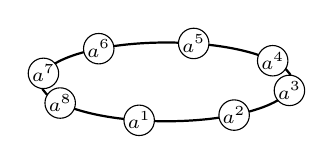
\begin{tikzpicture}[yscale=0.25, xscale=0.8]
      \draw[thick] (0,0) circle [radius=2];

      \node[spin, font=\scriptsize] at ({10-45/2}:2) {$a^3$};
      \node[spin, font=\scriptsize] at ({55-45/2}:2) {$a^4$};
      \node[spin, font=\scriptsize] at ({100-45/2}:2) {$a^5$};
      \node[spin, font=\scriptsize] at ({145-45/2}:2) {$a^6$};
      \node[spin, font=\scriptsize] at ({190-45/2}:2) {$a^7$};
      \node[spin, font=\scriptsize] at ({235-45/2}:2) {$a^8$};
      \node[spin, font=\scriptsize] at ({280-45/2}:2) {$a^1$};
      \node[spin, font=\scriptsize] at ({325-45/2}:2) {$a^2$};
    \end{tikzpicture}
  \end{equation*}

  Spins $a^1$, $\dotsc$, $a^n \in \hf^*$, \ $\hf$ = Cartan of $\slf_N$:
  \begin{equation*}
    a^r = \diag(a^r_1, \dotsc, a^r_N) \,,
    \qquad
    \sum_{i=1}^N a^r_i = 0
  \end{equation*}

  Local Hilbert space:
  $\CM_{\hf^*} = \{\text{meromorphic functions on $\hf^*$}\}$

  Total Hilbert space
  \begin{equation*}
    \CH
    =
    \underbrace{\CM_{\hf^*} \otimes \dotsb \otimes \CM_{\hf^*}}_n
  \end{equation*}
\end{frame}


\begin{frame}
  Equivalent lattice model
  \begin{equation*}
    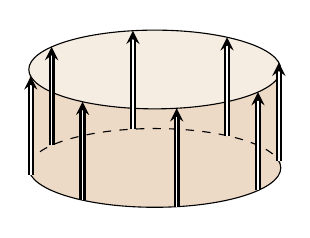
\begin{tikzpicture}[yscale=0.25, xscale=0.8]
      \fill[brown!30] (-2,0) arc (-180:0:2) -- +(0,5) arc (0:-180:2) --
      +(0,-5) -- cycle;
      \fill[brown!15]  (0,5) circle [radius=2];      

      \draw[dashed] (2,0) arc (0:180:2);
      \draw (-2,0) arc (180:360:2);
      \draw (0,5) circle [radius=2];
      
      \draw[thick, double, ->] (10:2) -- ++(90:5);
      \draw[thick, double, ->] (55:2) -- ++(90:5);
      \draw[thick, double, ->] (100:2) -- ++(90:5);
      \draw[thick, double, ->] (145:2) -- ++(90:5);
      \draw[thick, double, ->] (190:2) -- ++(90:5);
      \draw[thick, double, ->] (235:2) -- ++(90:5);
      \draw[thick, double, ->] (280:2) -- ++(90:5);
      \draw[thick, double, ->] (325:2) -- ++(90:5);
    \end{tikzpicture}
  \end{equation*}
  Spins live between double lines:
  \begin{equation*}
    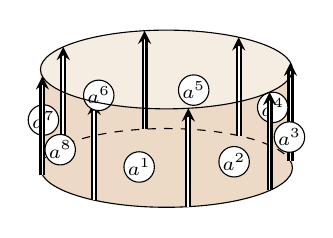
\begin{tikzpicture}[yscale=0.25, xscale=0.8]
      \fill[brown!30] (-2,0) arc (-180:0:2) -- +(0,5) arc (0:-180:2) --
      +(0,-5) -- cycle;
      \fill[brown!15]  (0,5) circle [radius=2];      

      \draw[dashed] (2,0) arc (0:180:2);
      \draw (-2,0) arc (180:360:2);
      
      \draw[thick, double, ->] (10:2) -- ++(90:5);
      \draw[thick, double, ->] (55:2) -- ++(90:5);
      \draw[thick, double, ->] (100:2) -- ++(90:5);
      \draw[thick, double, ->] (145:2) -- ++(90:5);
      \draw[thick, double, ->] (235:2) -- ++(90:5);
      \draw[thick, double, ->] (280:2) -- ++(90:5);

      \begin{scope}[shift={(0,2)}]
        \node[spin, font=\scriptsize] at ({10-45/2}:2) {$a^3$};
        \node[spin, font=\scriptsize] at ({55-45/2}:2) {$a^4$};
        \node[spin, font=\scriptsize] at ({100-45/2}:2) {$a^5$};
        \node[spin, font=\scriptsize] at ({145-45/2}:2) {$a^6$};
        \node[spin, font=\scriptsize] at ({190-45/2}:2) {$a^7$};
        \node[spin, font=\scriptsize] at ({235-45/2}:2) {$a^8$};
        \node[spin, font=\scriptsize] at ({280-45/2}:2) {$a^1$};
        \node[spin, font=\scriptsize] at ({325-45/2}:2) {$a^2$};
      \end{scope}

      \draw (0,5) circle [radius=2];
      \draw[thick, double, ->] (325:2) -- ++(90:5);

      \draw[thick, double, ->] (190:2) -- ++(90:5);
    \end{tikzpicture}
  \end{equation*}
  $a^r$ are called \alert{dynamical parameters}.
\end{frame}


\begin{frame}
  \alert{Transfer matrix} $T(z)$ is horizontal loop operator:
  \begin{equation*}
    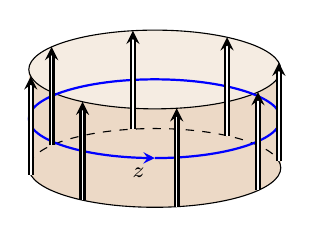
\begin{tikzpicture}[yscale=0.25, xscale=0.8]
      \fill[brown!30] (-2,0) arc (-180:0:2) -- +(0,5) arc (0:-180:2) --
      +(0,-5) -- cycle;
      \fill[brown!15]  (0,5) circle [radius=2];      

      \draw[dashed] (2,0) arc (0:180:2);
      \draw (-2,0) arc (180:360:2);
      \draw (0,5) circle [radius=2];
      
      \draw[blue, thick, ->] (-2,2.5) arc (-180:-90:2) node[black, below left] {$z$};
      \draw[blue, thick] (-2,2.5) arc (180:-90:2);
      
      \draw[thick, double, ->] (10:2) -- ++(90:5);
      \draw[thick, double, ->] (55:2) -- ++(90:5);
      \draw[thick, double, ->] (100:2) -- ++(90:5);
      \draw[thick, double, ->] (145:2) -- ++(90:5);
      \draw[thick, double, ->] (190:2) -- ++(90:5);
      \draw[thick, double, ->] (235:2) -- ++(90:5);
      \draw[thick, double, ->] (280:2) -- ++(90:5);
      \draw[thick, double, ->] (325:2) -- ++(90:5);
    \end{tikzpicture}
  \end{equation*}

  Solid line is worldline of particle whose Hilbert space is $\C^N$;
  its state changes when it crosses other lines.

  Solid line also has \alert{spectral parameter} $z \in \C$.

  $T(z)$ consists of $n$ copies of \alert{L-operator}
  \begin{equation*}
    L(z)
    =
    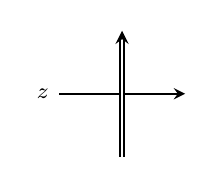
\begin{tikzpicture}[xscale=0.8, yscale=0.8, baseline=(x.base)]
      \node (x) at (0,0) {\vphantom{x}};
      
      \draw[thick, ->] (0,0) node[left] {$z$} -- (2,0);
      \draw[thick, double, ->] (1,-1) -- (1,1);
    \end{tikzpicture}
    \quad .
  \end{equation*}
\end{frame}


\begin{frame}
  Dynamical parameters jump across solid lines:
  \begin{equation*}
    L(z; a^1, a^2)_i^j
    =
    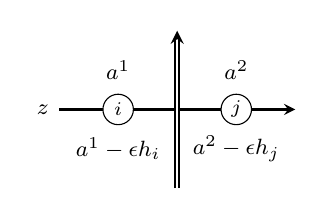
\begin{tikzpicture}[xscale=1.5, baseline=(x.base)]
      \node (x) at (0,0) {\vphantom{x}};
      
      \draw[thick, ->] (0,0) node[left] {$z$} -- (2,0);
      \draw[thick, double, ->] (1,-1) -- (1,1);
      
      \node at (0.5, 0.5) {$a^1$};
      \node at (1.5, 0.5) {$a^2$};
      \node at (0.5, -0.5) {$a^1 - \eps h_i$};
      \node at (1.5, -0.5) {$a^2 - \eps h_j$};
      \node[spin] at (0.5,0) {$i$};
      \node[spin] at (1.5,0) {$j$};
    \end{tikzpicture}
    \quad .
  \end{equation*}
  $\eps \in \C$ is a parameter,
  $h_1 = \diag(1-\tfrac1N, -\tfrac1N, \dotsc, -\tfrac1N)$, etc.

  Matrix elements $L(z)_i^j$ are difference operators on
  $\CM_{\hf^*} \otimes \CM_{\hf^*}$:
  \begin{equation*}
    L(z) = \sum_{i,j} L(z; a^1, a^2)_i^j \Delta_i^1 \Delta_j^2 \,,
    \qquad
    \Delta_i^r\colon a^r \mapsto a^r - \eps h_i \,.
  \end{equation*}

  Transfer matrix
  \begin{equation*}
    T(z)
    =
    \sum_{i^1, \dotsc, i^n}
    \prod_{r=1}^n
    L(z; a^r,a^{r+1})^{i^{r+1}}_{i^r}
    \prod_{s=1}^n \Delta_{i^s}^s \,,
    \qquad
    i^{n+1} = i^1
  \end{equation*}
  is a difference operator on $\CH = \CM_{\hf^*}^{\otimes n}$.
\end{frame}


\begin{frame}
  Crossing solid lines give \alert{R-matrix}
  \begin{equation*}
  R(z - z'; a)_{ij}^{kl}
  =
  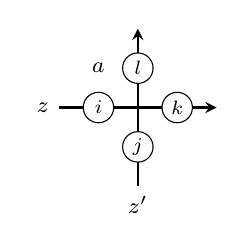
\begin{tikzpicture}[scale=1, baseline=(x.base)]
    \node (x) at (0,0) {\vphantom{x}};

    \draw[thick, ->] (0,0) node[left] {$z$} -- (2,0);
    \draw[thick, ->] (1,-1) node[below] {$z'$} -- (1,1);

    \node at (0.5, 0.5) {$a$};

    \node[spin] at (0.5,0) {$i$};
    \node[spin] at (1.5,0) {$k$};
    \node[spin] at (1,-0.5) {$j$};
    \node[spin] at (1,0.5) {$l$};
  \end{tikzpicture}
  \quad .
\end{equation*}
L-operator and R-matrix satisfy \alert{RLL relation}
\begin{equation*}
  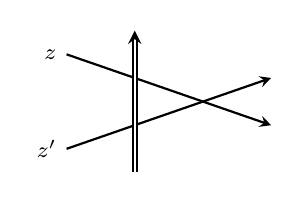
\begin{tikzpicture}[yscale=0.6, baseline=(x.base)]
      \node (x) at (30:2) {};
      
      \draw[thick, ->] (0,0) node[left] {$z'$} -- ++(30:3);
      \draw[thick, ->] (0,2) node[left] {$z$} -- ++(-30:3);
      \draw[thick, double, ->] (-30:1) -- ++(0,3);
    \end{tikzpicture}
    \ =
    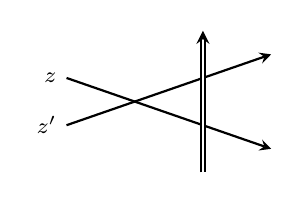
\begin{tikzpicture}[yscale=0.6, baseline=(x.base)]
      \node (x) at (30:1) {};
      
      \draw[thick, ->] (0,0) node[left] {$z'$} -- ++(30:3);
      \draw[thick, ->] (0,1) node[left] {$z$} -- ++(-30:3);
      \draw[thick, double, ->] (-30:2) -- ++(0,3);
    \end{tikzpicture}
    \quad .
  \end{equation*}
  Also, R-matrix satisfies dynamical Yang--Baxter equation.
\end{frame}


\begin{frame}
  From RLL relation it follows that transfer matrices commute:
  \begin{equation*}
    T(z) T(z') = T(z') T(z)
  \end{equation*}
  \begin{equation*}
    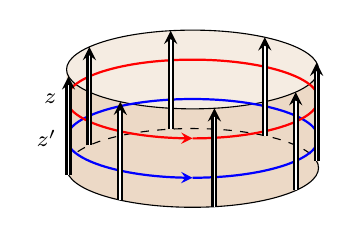
\begin{tikzpicture}[yscale=0.25, xscale=0.8, baseline=(x.base)]
      \node (x) at (0,2.5) {};

      \fill[brown!30] (-2,0) arc (-180:0:2) -- +(0,5) arc (0:-180:2) --
      +(0,-5) -- cycle;
      \fill[brown!15]  (0,5) circle [radius=2];      

      \draw[dashed] (2,0) arc (0:180:2);
      \draw (-2,0) arc (180:360:2);
      \draw (0,5) circle [radius=2];
      
      \draw[blue, thick, ->] (-2,1.5)  node[black, left] {$z'$} arc (-180:-90:2);
      \draw[blue, thick] (-2,1.5) arc (180:-90:2);
      
      \draw[red, thick, ->] (-2,3.5) node[black, left] {$z$} arc (-180:-90:2);
      \draw[red, thick] (-2,3.5) arc (180:-90:2);
      
      \draw[thick, double, ->] (10:2) -- ++(90:5);
      \draw[thick, double, ->] (55:2) -- ++(90:5);
      \draw[thick, double, ->] (100:2) -- ++(90:5);
      \draw[thick, double, ->] (145:2) -- ++(90:5);
      \draw[thick, double, ->] (190:2) -- ++(90:5);
      \draw[thick, double, ->] (235:2) -- ++(90:5);
      \draw[thick, double, ->] (280:2) -- ++(90:5);
      \draw[thick, double, ->] (325:2) -- ++(90:5);
    \end{tikzpicture}
    \
    =
    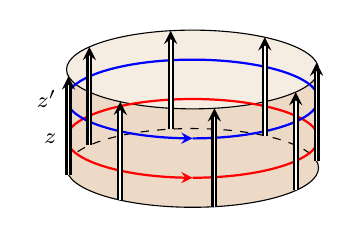
\begin{tikzpicture}[yscale=0.25, xscale=0.8, baseline=(x.base)]
      \node (x) at (0,2.5) {};

      \fill[brown!30] (-2,0) arc (-180:0:2) -- +(0,5) arc (0:-180:2) --
      +(0,-5) -- cycle;
      \fill[brown!15]  (0,5) circle [radius=2];      

      \draw[dashed] (2,0) arc (0:180:2);
      \draw (-2,0) arc (180:360:2);
      \draw (0,5) circle [radius=2];
      
      \draw[red, thick, ->] (-2,1.5)  node[black, left] {$z$} arc (-180:-90:2);
      \draw[red, thick] (-2,1.5) arc (180:-90:2);
      
      \draw[blue, thick, ->] (-2,3.5) node[black, left] {$z'$} arc (-180:-90:2);
      \draw[blue, thick] (-2,3.5) arc (180:-90:2);
      
      \draw[thick, double, ->] (10:2) -- ++(90:5);
      \draw[thick, double, ->] (55:2) -- ++(90:5);
      \draw[thick, double, ->] (100:2) -- ++(90:5);
      \draw[thick, double, ->] (145:2) -- ++(90:5);
      \draw[thick, double, ->] (190:2) -- ++(90:5);
      \draw[thick, double, ->] (235:2) -- ++(90:5);
      \draw[thick, double, ->] (280:2) -- ++(90:5);
      \draw[thick, double, ->] (325:2) -- ++(90:5);
    \end{tikzpicture}
  \end{equation*}



  % Proof:
  % \begin{equation*}
  %   \begin{tikzpicture}[yscale=0.6, baseline=(x.base)]
  %     \node (x) at (0,0.5) {\vphantom{x}};
      
  %     \draw[thick, ->, rounded corners] (0,0) node[left] {$z'$} -- (2.5,0) -- (3,1) -- (3.5,1);
  %     \draw[thick, ->, rounded corners] (0,1) node[left] {$z$} -- (2.5,1) -- (3,0) -- (3.5,0);

  %     \draw[thick, double, ->] (0.5,-1) -- +(90:3);
  %     \draw[thick, double, ->] (1,-1) -- +(90:3);
  %     \draw[thick, double, ->] (2,-1) -- +(90:3);

  %     \node at (1.5,-0.5) {$\dots$};
  %   \end{tikzpicture}
  %   \ =
  %   \begin{tikzpicture}[yscale=0.6, baseline=(x.base)]
  %     \node (x) at (0,0.5) {\vphantom{x}};
      
  %     \draw[thick, ->, rounded corners] (0,0) node[left] {$z'$} -- (0.5,0) -- (1,1) -- (3.5,1);

  %     \draw[thick, ->, rounded corners] (0,1) node[left] {$z$} -- (0.5,1) -- (1,0) -- (3.5,0);


  %     \draw[thick, double, ->] (1.5,-1) -- +(90:3);
  %     \draw[thick, double, ->] (2,-1) -- +(90:3);
  %     \draw[thick, double, ->] (3,-1) -- +(90:3);

  %     \node at (2.5,-0.5) {$\dots$};
  %   \end{tikzpicture}
  % \end{equation*}
  % by RLL relation.  Multiply both sides by $R^{-1}$ and take the trace.

  Coefficients of Laurent expansion
  \begin{equation*}
    T(z) = \sum_{m=-\infty}^\infty T_m z^m
  \end{equation*}
  are commuting difference operators on $\CH$:
  \begin{equation*}
    [T_m, T_n] = 0 \,.
  \end{equation*}
  This is \alert{integrability}.
\end{frame}


\begin{frame}
  Trigonometric L-operator
  \begin{equation*}
    \CL_{w,m}(z)_i^j
    =
    \sum_{i,j}
    (\Delta^1_i \Delta^2_j)^{\frac12}
    \frac{\sin\pi(z - w + a^2_j - a^1_i)}{\sin\pi(z - w)}
    \ell_m(a^1, a^2)_i^j
    (\Delta^1_i \Delta^2_j)^{\frac12}
  \end{equation*}
  satisfies RLL relation with trigonometric dynamical R-matrix.

  $w$, $m \in \C$ are spectral parameters assigned to double line and
  \begin{equation*}
    \ell_m(a^1, a^2)_i^j
    =
    \Biggl(
    \frac{\prod_{k (\neq i)} \sin\pi(a^1_k - a^2_j - m)
      \prod_{l (\neq j)} \sin\pi(a^1_i - a^2_l - m)}
    {\prod_{k (\neq i)}\sin\pi(a^1_{ki} - \frac12\eps)
      \sin\pi(a^1_{ik} - \frac12\eps)}
    \Biggr)^{\frac12} \,.
  \end{equation*}
\end{frame}


\begin{frame}
  Introduce \alert{fundamental L-operators}
  \begin{equation*}
    \CL_{\pm,m} = \lim_{w \to \pm\iu\infty} \CL_{w,m} \,.
  \end{equation*}
  Then
  \begin{equation*}
    (\CL_{\pm,m})_i^j
    =
    \sum_{i,j}
    (\Delta^1_i \Delta^2_j)^{\frac12}
    e^{\pm\pi\iu(a^2_j - a^1_i)}
    \ell_m(a^1, a^2)_i^j
    (\Delta^1_i \Delta^2_j)^{\frac12}
  \end{equation*}
  and
  \begin{equation*}
    \CL_{w,m}(z)
    =
    \frac{e^{\pi\iu(z-w)} \CL_{+,m} - e^{-\pi\iu(z-w)} \CL_{-,m}}{\sin\pi(z-w)}
    \,.
  \end{equation*}
  
  For $\sigma \in \{\pm\}^n$ and $m \in \C^n$, let $\CT_{\sigma,m}$ be
  the transfer matrix constructed from $\CL_{\sigma^1,m^1}$, $\dotsc$,
  $\CL_{\sigma^n,m^n}$:
  \begin{equation*}
    \CT_{\sigma,m}
    =
    \sum_{i^1, \dotsc, i^n}
    \Biggl(\prod_{s=1}^n \Delta^s_{i_s}\Biggr)^{\frac12}
    \prod_{r=1}^n
    e^{\pi\iu\sigma^r (a^{r+1}_{i^{r+1}} - a^r_{i^r})}
    \ell_{m^r}(a^r, a^{r+1})_{i^r}^{i^{r+1}}
    \Biggl(\prod_{s=1}^n \Delta^s_{i_s}\Biggr)^{\frac12}
    \,.
  \end{equation*}
\end{frame}


\section*{Gauge theory side}

\begin{frame}
  $\CN = 2$ gauge theories have half-BPS \alert{Wilson--'t Hooft lines}.

  Wolrdlines of very massive dyonic particles

  Charge of Wilson--'t Hooft line
  \begin{equation*}
    (\mcharge, \echarge)
    \in (\Lambda_{\text{coweight}} \times \Lambda_{\text{weight}})/\mathrm{Weyl} \,.
  \end{equation*}

  Wilson line has $\mcharge = 0$ and is labeled by representation of $\gf$.

  't Hooft line has $\echarge = 0$ and is labeled by representation of ${}^L\gf$.

  Wilson--'t Hooft \\
  = ('t Hooft) + (Wilson for subgroup of $G$ leaving $\mcharge$ invariant)
\end{frame}


\begin{frame}
  $\CN = 2$ gauge theory described by $n$-node \alert{circular quiver}
  \begin{equation*}
    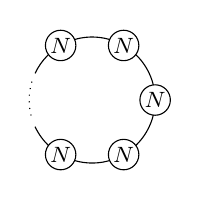
\begin{tikzpicture}[scale=0.8, baseline=(x.base)]
      \node (x) at (0,0) {\vphantom{x}};
      
      \draw[dotted] (163:1) arc (163:197:1);
      \draw (-155:1) arc (-155:155:1);
      
      \node[gnode] at (0:1) {$N$};
      \node[gnode] at (60:1) {$N$};
      \node[gnode] at (120:1) {$N$};
      \node[gnode] at (240:1) {$N$};
      \node[gnode] at (300:1) {$N$};
    \end{tikzpicture}
  \end{equation*}
  Each node is $\SU(N)$.

  Edges are bifundamental hypers with masses $m^1$, $\dotsc$, $m^n$.

  Compactification of 6d $\CN = (2,0)$ SCFT on $n$-punctured torus
  \begin{equation*}
  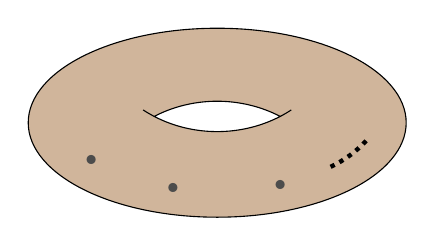
\begin{tikzpicture}[scale=0.8]

    % Taubmans Cinnamon Doughnut color
    \draw[fill={rgb,255:red,208; green,181; blue,155},even odd rule]
    (0,0) ellipse (3 and 1.5) 
    (-1,0.1) arc (120:60:2 and 1.8) arc (-60:-120:2 and 1.8);

    \draw (-1,0.1) arc(-120:-126:2 and 1.8) (1,0.1) arc(-60:-54:2 and 1.8);

    % \node[black!60] (p1) at (-1,-1) {$\bullet$};
    % \node[black!60] (p2) at (0.7,-1.05) {$\bullet$};
    % \node[black!60] (p3) at (2,-0.6) {$\bullet$};

    \node[black!70] (p3) at (1,-1) {$\bullet$};
    \node[black!70] (p2) at (-0.7,-1.05) {$\bullet$};
    \node[black!70] (p1) at (-2,-0.6) {$\bullet$};


    \draw[ultra thick, dotted] (1.8,-0.7) arc (-65:-42:1.8);
  \end{tikzpicture}
\end{equation*}
\end{frame}


\begin{frame}
  Wilson--'t Hooft lines come from surface operators wrapping 1-cycles
  on the torus.
  \begin{equation*}
    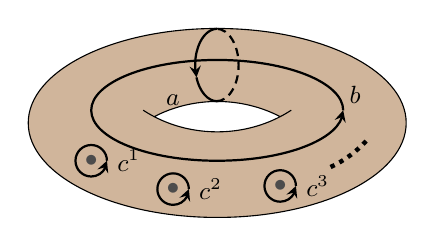
\begin{tikzpicture}[font=\small, scale=0.8]
      
      % Taubmans Cinnamon Doughnut color
      \draw[fill={rgb,255:red,208; green,181; blue,155},even odd rule]
      (0,0) ellipse (3 and 1.5) 
      (-1,0.1) arc (120:60:2 and 1.8) arc (-60:-120:2 and 1.8);
      
      \draw (-1,0.1) arc(-120:-126:2 and 1.8) (1,0.1) arc(-60:-54:2 and 1.8);
      
      \draw[thick, ->] (2,0.2) arc (0:360:2 and 0.8) node[above right=-2pt] {$b$};
      
      \draw[thick, ->] (0,1.495)
      node[shift={(-16pt,-0.9)}] {$a$} arc (90:200:0.35 and 0.575);
      \draw[thick] (-0.33,0.7235) arc (200:270:0.35 and 0.575);
      \draw[thick, densely dashed] (-0.01,0.345) arc (270:450:0.35 and 0.575);
      
      % \node[black!60] (p1) at (-1,-1) {$\bullet$};
      % \node[black!60] (p2) at (0.7,-1.05) {$\bullet$};
      % \node[black!60] (p3) at (2,-0.6) {$\bullet$};
      
      \node[black!70] (p3) at (1,-1) {$\bullet$};
      \node[black!70] (p2) at (-0.7,-1.05) {$\bullet$};
      \node[black!70] (p1) at (-2,-0.6) {$\bullet$};
      
      
      \draw[ultra thick, dotted] (1.8,-0.7) arc (-65:-42:1.8);
      
      \draw[thick, ->] ($(p1)+(0.25,0)$) arc (0:360:0.25) node[right] {$c^1$};
      \draw[thick, ->] ($(p2)+(0.25,0)$) arc (0:360:0.25) node[right] {$c^2$};
      \draw[thick, ->] ($(p3)+(0.25,0)$) arc (0:360:0.25) node[right] {$c^3$};
    \end{tikzpicture}
  \end{equation*}

  Consider Wilson--'t Hooft line $T_{\square,\sigma}$ corresponding to
  \begin{equation*}
    \gamma_\sigma
    =
    b + \sum_r \frac{1 - \sigma^r}{2} c^r \,.
  \end{equation*}
  If $\sigma^r = +1$ ($-1$), the cycle passes above (below) $r$th
  puncture.
  
  It has
  \begin{equation*}
    \mcharge = \square \oplus \dotsb \oplus \square
  \end{equation*}
  under ${}^L\suf_N \oplus \dotsb \oplus {}^L\suf_N$, and $\echarge$
  specified by $\sigma \in \{\pm\}^n$.
  
  % This breaks $\SU(N)^n \to \mathrm{S}(\U(1) \times \U(N-1))^n$.

  % Turn on Wilson line which, under the $\U(1)$s, has charge
  % \begin{equation*}
  %   E = \sum_{r=1}^n \frac12 (\sigma^r - \sigma^{r+1})
  %   =
  %   \begin{cases}
  %     0 & (\sigma^r = \sigma^{r+1} = \pm 1) \\
  %     +1 & (\sigma^r = -\sigma^{r+1} = +1) \\
  %     -1 & (\sigma^r = -\sigma^{r+1} = -1)
  %   \end{cases}
  % \end{equation*}
\end{frame}




\begin{frame}
  Put the theory on twisted product $S^1 \times_\eps \R^2 \times \R$.

  Wrap $T_{\square,\sigma}$ around $S^1 \times \{0\} \times \{t\}$.

  Ito--Okuda--Taki tell us how to compute the vev by localization:
  \begin{equation*}
    \vev{T_{\square, \sigma}}
    =
    \sum_{i^1, \dotsc, i^n}
    \prod_{r=1}^n
    e^{2\pi\iu b^r_{i^r}}
    e^{\pi\iu\sigma^r (a^{r+1}_{i^{r+1}} - a^r_{i^r})}
    \ell_{m^r}(a^r, a^{r+1})_{i^r}^{i^{r+1}}
    \,,
  \end{equation*}
  where
  \begin{equation*}
    a^r = R(A^r_0 + i\phi^r_0)(\infty) \,,
    \qquad
    b^r = \frac{\Theta^r}{2\pi} - \frac{4\pi\iu R}{g^2} \phi^r_9(\infty)
  \end{equation*}
  $\Theta^r$ are magnetic Wilson lines around $S^1$.

  Alternatively, we can compute it from Toda theory.
\end{frame}



\section*{Correspondence}

\begin{frame}
  Compare
  \begin{equation*}
    \vev{T_{\square, \sigma}}
    =
    \sum_{i^1, \dotsc, i^n}
    \prod_{r=1}^n
    e^{2\pi\iu b^r_{i^r}}
    e^{\pi\iu\sigma^r (a^{r+1}_{i^{r+1}} - a^r_{i^r})}
    \ell_{m^r}(a^r, a^{r+1})_{i^r}^{i^{r+1}} \,,
  \end{equation*}
  \begin{equation*}
    \CT_{\sigma,m}
    =
    \sum_{i^1, \dotsc, i^n}
    \Biggl(\prod_{s=1}^n \Delta^s_{i_s}\Biggr)^{\frac12}
    \prod_{r=1}^n
    e^{\pi\iu\sigma^r (a^{r+1}_{i^{r+1}} - a^r_{i^r})}
    \ell_{m^r}(a^r, a^{r+1})_{i^r}^{i^{r+1}}
    \Biggl(\prod_{s=1}^n \Delta^s_{i_s}\Biggr)^{\frac12}
    \,.
  \end{equation*}
  If we quantize $a^r$, $b^r$ so that
  \begin{equation*}
    [\ah^r_i, \bh^s_j]
    = -\iu \frac{\eps}{2\pi} \delta^{rs} \biggl(\delta_{ij} - \frac1N\biggr) \,,
  \end{equation*}
  then
  \begin{equation*}
    \CT_{\sigma,m}
    = \text{Weyl quantization of $\vev{T_{\square, \sigma}}$} \,.
  \end{equation*}
\end{frame}



\section*{Brane realization}

\begin{frame}
  M-theory setup
  \begin{equation*}
    \begin{tabular}{rcccccccccc}
      Spacetime & $\R_0$ & $\R^2_{12}$ & $S^1_3$ & $\R^2_{45}$ & $S^1_6$
      & $\R_7$ & $\R_8$ & $\R_9$ & $S^1_{10}$
      \\
      $N$ M5 & $\R_0$ & $\R^2_{12}$ & $S^1_3$ & $-$ & $S^1_6$
      & $-$ & $-$ & $-$ & $S^1_{10}$
     \\
      $n$ M5$'$ & $\R_0$ & $\R^2_{12}$ & $S^1_3$ & $-$
      & $-$ & $-$ & $\R_8$ & $\R_9$ & $-$
     \\
      M2 & $-$ & $-$ & $S^1_3$ & $-$ & $S^1_6$
      & $-$ & $\R^{\geq 0}_8$ & $-$ & $-$
    \end{tabular}
  \end{equation*}

  12345 directions: twisted product
  $\R^2_{12} \times_\eps S^1_3 \times_{-\eps} \R^2_{45}$

  M5: 6d $\CN = (2,0)$ SCFT of type $\suf_N$ on
  $\R_0 \times \R^2_{12} \times_\eps S^1_3 \times S^1_6 \times
  S^1_{10}$

  M5$'$: $n$ punctures on $S^1_6 \times S^1_{10}$

  M2: surface operator

  Reduction on $S^1_6 \times S^1_{10}$ gives the 4d setup with
  $\sigma = (+,\dotsc,+)$.
\end{frame}


\begin{frame}
  \begin{equation*}
    \begin{tabular}{rcccccccccc}
      Spacetime & $\R_0$ & $\R^2_{12}$ & $S^1_3$ & $\R^2_{45}$ & $S^1_6$
      & $\R_7$ & $\R_8$ & $S^1_9$ & $S^1_{10}$
      \\
      $N$ M5 & $\R_0$ & $\R^2_{12}$ & $S^1_3$ & $-$ & $S^1_6$
      & $-$ & $-$ & $-$ & $S^1_{10}$
     \\
      $n$ M5$'$ & $\R_0$ & $\R^2_{12}$ & $S^1_3$ & $-$
      & $-$ & $-$ & $\R_8$ & $S^1_9$ & $-$
     \\
      M2 & $-$ & $-$ & $S^1_3$ & $-$ & $S^1_6$
      & $-$ & $\R^{\geq 0}_8$ & $-$ & $-$
    \end{tabular}
  \end{equation*}

  Compactify $\R_9 \to S^1_9$.

  Reduce on $S^1_3$ and apply T-duality $S^1_9 \to \check S^1_9$:
  \begin{equation*}
    \begin{tabular}{rccccccccc}
      Spacetime & $\R_0$ & $\R^2_{12}$ & $\R^2_{45}$ & $S^1_6$
      & $\R_7$ & $\R_8$ & $\check S^1_9$ & $S^1_{10}$
      \\
      $N$ D5 & $\R_0$ & $\R^2_{12}$ & $-$ & $S^1_6$
      & $-$ & $-$ & $\check S^1_9$ & $S^1_{10}$
     \\
      $n$ D3 & $\R_0$ & $\R^2_{12}$ & $-$
      & $-$ & $-$ & $\R_8$ & $-$
     \\
      F1 & $-$ & $-$ & $-$ & $S^1_6$
      & $-$ & $\R^{\geq 0}_8$ & $-$ & $-$
    \end{tabular}
  \end{equation*}
\end{frame}

\begin{frame}
    \begin{equation*}
    \begin{tabular}{rccccccccc}
      Spacetime & $\R_0$ & $\R^2_{12}$ & $\R^2_{45}$ & $S^1_6$
      & $\R_7$ & $\R_8$ & $\check S^1_9$ & $S^1_{10}$
      \\
      $N$ D5 & $\R_0$ & $\R^2_{12}$ & $-$ & $S^1_6$
      & $-$ & $-$ & $\check S^1_9$ & $S^1_{10}$
     \\
      $n$ D3 & $\R_0$ & $\R^2_{12}$ & $-$
      & $-$ & $-$ & $\R_8$ & $-$
     \\
      F1 & $-$ & $-$ & $-$ & $S^1_6$
      & $-$ & $\R^{\geq 0}_8$ & $-$ & $-$
    \end{tabular}
  \end{equation*}

  D5: 6d $\CN = (1,1)$ SYM on
  $\R_0 \times \R^2_{12} \times S^1_6 \times \check S^1_9 \times S^1_{10}$

  D3: codim-3 operator on $\R_0 \times \R^2_{12}$

  F1: Wilson line on $S^1_6$

  $\Omega$-deformation on $\R^2_{12}$ due to the twisted product
  \begin{equation*}
    \R^2_{12} \times_\eps S^1_3 \times_{-\eps} \R^2_{45}
  \end{equation*}
\end{frame}

\begin{frame}
  $\Omega$-deformation of 6d $\CN = (1,1)$ SYM on
  $\R_0 \times \R^2_{12} \times S^1_6 \times \check S^1_9 \times S^1_{10}$ \\[1ex]
  \quad $\rightsquigarrow$ Costello's 4d Chern--Simons on
  $\R_0 \times S^1_6 \times \check S^1_9 \times S^1_{10}$
  \cite{Costello--Y}

  Codim-3 operators on $\R_0 \times \R^2_{12}$ \\[1ex]
  \quad $\rightsquigarrow$ line operators on $\R_0$

  Wilson line on $S^1_6$ \\[1ex]
  \quad $\rightsquigarrow$ Wilson line on $S^1_6$

  \begin{equation*}
    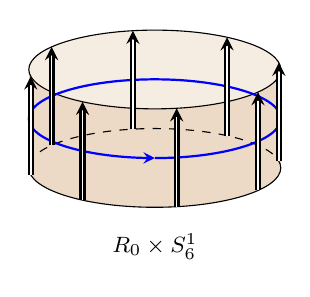
\begin{tikzpicture}[yscale=0.25, xscale=0.8, baseline=(x.base)]
      \node (x) at (0,2.5) {\vphantom{x}};

      \fill[brown!30] (-2,0) arc (-180:0:2) -- +(0,5) arc (0:-180:2) --
      +(0,-5) -- cycle;
      \fill[brown!15]  (0,5) circle [radius=2];      

      \draw[dashed] (2,0) arc (0:180:2);
      \draw (-2,0) arc (180:360:2);
      \draw (0,5) circle [radius=2];
      
      \draw[blue, thick, ->] (-2,2.5) arc (-180:-90:2);
      \draw[blue, thick] (-2,2.5) arc (180:-90:2);
      
      \draw[thick, double, ->] (10:2) -- ++(90:5);
      \draw[thick, double, ->] (55:2) -- ++(90:5);
      \draw[thick, double, ->] (100:2) -- ++(90:5);
      \draw[thick, double, ->] (145:2) -- ++(90:5);
      \draw[thick, double, ->] (190:2) -- ++(90:5);
      \draw[thick, double, ->] (235:2) -- ++(90:5);
      \draw[thick, double, ->] (280:2) -- ++(90:5);
      \draw[thick, double, ->] (325:2) -- ++(90:5);

      \node at (0,-4) {$\R_0 \times S^1_6$};
    \end{tikzpicture}
    \quad \times \quad
    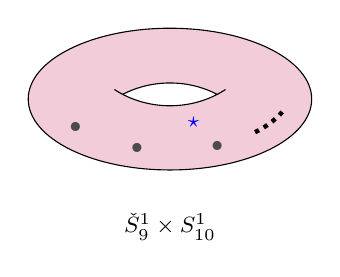
\begin{tikzpicture}[scale=0.6, baseline=(x.base)]
      \node (x) at (0,0) {\vphantom{x}};

      \draw[fill=purple!20,even odd rule]
      (0,0) ellipse (3 and 1.5) 
      (-1,0.1) arc (120:60:2 and 1.8) arc (-60:-120:2 and 1.8);
      
      \draw (-1,0.1) arc(-120:-126:2 and 1.8) (1,0.1) arc(-60:-54:2 and 1.8);

      \node[black!70] (p3) at (1,-1) {$\bullet$};
      \node[black!70] (p2) at (-0.7,-1.05) {$\bullet$};
      \node[black!70] (p1) at (-2,-0.6) {$\bullet$};
      
      \node[blue] at (0.5,-0.5) {$\mathbf{\star}$};
      
      \draw[ultra thick, dotted] (1.8,-0.7) arc (-65:-42:1.8);

      \node at (0,-2.7) {$\check S^1_9 \times S^1_{10}$};
    \end{tikzpicture}
  \end{equation*}
\end{frame}

\begin{frame}
  \begin{equation*}
    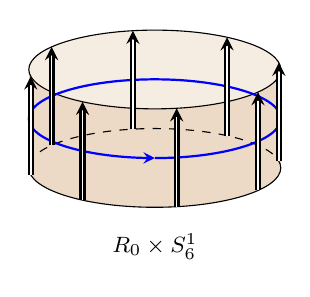
\begin{tikzpicture}[yscale=0.25, xscale=0.8, baseline=(x.base)]
      \node (x) at (0,2.5) {\vphantom{x}};

      \fill[brown!30] (-2,0) arc (-180:0:2) -- +(0,5) arc (0:-180:2) --
      +(0,-5) -- cycle;
      \fill[brown!15]  (0,5) circle [radius=2];      

      \draw[dashed] (2,0) arc (0:180:2);
      \draw (-2,0) arc (180:360:2);
      \draw (0,5) circle [radius=2];
      
      \draw[blue, thick, ->] (-2,2.5) arc (-180:-90:2);
      \draw[blue, thick] (-2,2.5) arc (180:-90:2);
      
      \draw[thick, double, ->] (10:2) -- ++(90:5);
      \draw[thick, double, ->] (55:2) -- ++(90:5);
      \draw[thick, double, ->] (100:2) -- ++(90:5);
      \draw[thick, double, ->] (145:2) -- ++(90:5);
      \draw[thick, double, ->] (190:2) -- ++(90:5);
      \draw[thick, double, ->] (235:2) -- ++(90:5);
      \draw[thick, double, ->] (280:2) -- ++(90:5);
      \draw[thick, double, ->] (325:2) -- ++(90:5);

      \node at (0,-4) {$\R_0 \times S^1_6$};
    \end{tikzpicture}
    \quad \times \quad
    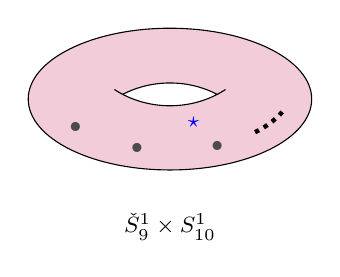
\begin{tikzpicture}[scale=0.6, baseline=(x.base)]
      \node (x) at (0,0) {\vphantom{x}};

      \draw[fill=purple!20,even odd rule]
      (0,0) ellipse (3 and 1.5) 
      (-1,0.1) arc (120:60:2 and 1.8) arc (-60:-120:2 and 1.8);
      
      \draw (-1,0.1) arc(-120:-126:2 and 1.8) (1,0.1) arc(-60:-54:2 and 1.8);

      \node[black!70] (p3) at (1,-1) {$\bullet$};
      \node[black!70] (p2) at (-0.7,-1.05) {$\bullet$};
      \node[black!70] (p1) at (-2,-0.6) {$\bullet$};
      
      \node[blue] at (0.5,-0.5) {$\mathbf{\star}$};
      
      \draw[ultra thick, dotted] (1.8,-0.7) arc (-65:-42:1.8);

      \node at (0,-2.7) {$\check S^1_9 \times S^1_{10}$};
    \end{tikzpicture}
  \end{equation*}

  Topological on $\R_0 \times S^1_6$, holomorphic on
  $\check S^1_9 \times S^1_{10}$

  Wilson line gives transfer matrix of elliptic QIS with
  \begin{equation*}
    \tau = \iu R_{10}/\check R_9 \,.
  \end{equation*}

  Now, decompactify $S^1_9 \to \R_9$.  Take $R_9 \to \infty$, or
  $\check R_9 \to 0$.
  
  This is the \alert{trigonometric limit} $\tau \to \iu\infty$.
\end{frame}

\begin{frame}
  \begin{equation*}
    \begin{tabular}{rccccccccc}
      Spacetime & $\R_0$ & $\R^2_{12}$ & $\R^2_{45}$ & $S^1_6$
      & $\R_7$ & $\R_8$ & $\check S^1_9$ & $S^1_{10}$
      \\
      $N$ D5 & $\R_0$ & $\R^2_{12}$ & $-$ & $S^1_6$
      & $-$ & $-$ & $\check S^1_9$ & $S^1_{10}$
     \\
      $n$ D3 & $\R_0$ & $\R^2_{12}$ & $-$
      & $-$ & $-$ & $\R_8$ & $-$ & $-$
     \\
      F1 & $-$ & $-$ & $-$ & $S^1_6$
      & $-$ & $\R^{\geq 0}_8$ & $-$ & $-$
    \end{tabular}
  \end{equation*}
  For Nekrasov--Shatashvili, apply S-duality and T-duality on $S^1_6$:
  \begin{equation*}
    \begin{tabular}{rccccccccc}
      Spacetime & $\R_0$ & $\R^2_{12}$ & $\R^2_{45}$ & $\check S^1_6$
      & $\R_7$ & $\R_8$ & $\check S^1_9$ & $S^1_{10}$
      \\
      $N$ NS5 & $\R_0$ & $\R^2_{12}$ & $-$ & $\check S^1_6$
      & $-$ & $-$ & $\check S^1_9$ & $S^1_{10}$
     \\
      $n$ D4 & $\R_0$ & $\R^2_{12}$ & $-$ & $\check S^1_6$
      & $-$ & $\R_8$ & $-$ & $-$
     \\
      D0 & $-$ & $-$ & $-$ & $-$
      & $-$ & $\R^{\geq 0}_8$ & $-$ & $-$
    \end{tabular}
  \end{equation*}

  D4--NS5: 4d $\CN = 2$ theory for $(N+1)$-node linear quiver
  \begin{equation*}
    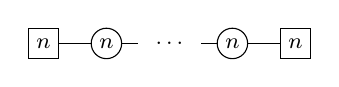
\begin{tikzpicture}[scale=0.8, baseline=(x.base)]
      \node (x) at (0,0) {\vphantom{x}};
      
      \node[fnode] (1) at (0,0) {$n$};
      \node[gnode] (2) at (1,0) {$n$};
      \node[gnode] (3) at (3,0) {$n$};
      \node[fnode] (4) at (4,0) {$n$};

      \draw (1) -- (2) -- +(0:0.5);
      \draw (4) -- (3) -- +(180:0.5);
      \node at (2,0) {$\dots$};
    \end{tikzpicture}
  \end{equation*}
  from which noncompact XXX spin chain arises.

  More precisely, 6d lift of this theory, hence elliptic.
\end{frame}


\begin{frame}
  Go back to M-theory
  \begin{equation*}
    \begin{tabular}{rcccccccccc}
      Spacetime & $\R_0$ & $\R^2_{12}$ & $S^1_3$ & $\R^2_{45}$ & $S^1_6$
      & $\R_7$ & $\R_8$ & $S^1_9$ & $S^1_{10}$
      \\
      $N$ M5 & $\R_0$ & $\R^2_{12}$ & $S^1_3$ & $-$ & $S^1_6$
      & $-$ & $-$ & $-$ & $S^1_{10}$
     \\
      $n$ M5$'$ & $\R_0$ & $\R^2_{12}$ & $S^1_3$ & $-$
      & $-$ & $-$ & $\R_8$ & $S^1_9$ & $-$
     \\
      M2 & $-$ & $-$ & $S^1_3$ & $-$ & $S^1_6$
      & $-$ & $\R^{\geq 0}_8$ & $-$ & $-$
    \end{tabular}
  \end{equation*}
  Reduce on $S^1_9$, apply T-duality on $S^1_{10}$ and S-duality:
    \begin{equation*}
    \begin{tabular}{rccccccccc}
      Spacetime & $\R_0$ & $\R^2_{12}$ & $S^1_3$ & $\R^2_{45}$ & $S^1_6$
      & $\R_7$ & $\R_8$ & $\check S^1_{10}$
      \\
      $N$ D5 & $\R_0$ & $\R^2_{12}$ & $S^1_3$ & $-$ & $S^1_6$
      & $-$ & $-$ & $\check S^1_{10}$
     \\
      $n$ NS5 & $\R_0$ & $\R^2_{12}$ & $S^1_3$ & $-$
      & $-$ & $-$ & $\R_8$ & $\check S^1_{10}$
     \\
      D3 & $-$ & $-$ & $S^1_3$ & $-$ & $S^1_6$
      & $-$ & $\R^{\geq 0}_8$ & $\check S^1_{10}$
    \end{tabular}
  \end{equation*}
  We can add NS5s in
  $\R^2_{12} \times_\eps S^1_3 \times S^1_6 \times \R_7 \times \check
  S^1_{10}$, preserving $\CN = 1$ SUSY on
  $\R^2_{12} \times_\eps S^1_3 \times \check S^1_{10}$.

  This is brane tiling with surface defect on
  $S^1_3 \times \check S^1_{10}$.
\end{frame}


\section*{Summary}

\begin{frame}
  Summary
  \begin{itemize}
  \item We considered a class of Wilson--'t Hooft lines in 4d
    $\CN = 2$ circular quiver theories.

  \item We found that they can be identified with transfer matrices of
    trigonometric QIS.

  \item By embedding into string theory, this correspondence can be
    related to other known correspondences via string dualities.
  \end{itemize}

  Further directions
  \begin{itemize}
  \item Wilson--'t Hooft lines in 5d circular quiver theory correspond
    to transfer matrices of elliptic QIS.

  \item Circular quiver theories deconstruct 6d $\CN = (2,0)$ SCFT.
    Integrability is behind surface operators in 6d theory.
  \end{itemize}
\end{frame}

\end{document}